%
% <LATEXTEMPLATE> Florian Wilhelm
% Erstellt am <DATUM>
%
% Bauen mit dem beiliegenden Makefile



\documentclass[11pt,a4paper,titlepage,ngerman]{article}

% Deutsch mit neuer Rechtschreibung
\usepackage[ngerman]{babel}

% Umlaute direkt eingeben http://www.jr-x.de/publikationen/latex/tipps/besonderheiten.html
% Hatte hier ursprünglich "latin1" als Option, das ging aber nicht. Hängt wohl von der Codierung des Dokumentes ab.
\usepackage[utf8]{inputenc} 

% Einbinden von Grafiken
\usepackage{graphicx}

% Syntax-Highliting für Quelltext
% Benötigt die zusätzlichen Optionen "-shell-escape -interaction=nonstopmode" zum bauen.
\usepackage{minted} 

% Setzen der Eigenschaften der erzeugten PDF-Datei
% TODO: Immer schön anpassen!
\usepackage[pdftex,
    pdfauthor={Florian Wilhelm},
    pdfsubject={<LATEXTEMPLATE>},
    pdftitle={<LATEXTEMPLATE>},    
    pdfproducer={Latex with hyperref},
    pdfcreator={pdflatex}]{hyperref}

% Glossar-Paket laden und Glossar erzeugen
% Hierfür sind mehrere Übersetzungsvorgänge nötig. Dafür gibt es ein Build-Target im Makefile.
\usepackage[toc]{glossaries}
\makeglossaries

%
% Glossar
%
\newglossaryentry{lorem}{name={LOREM GALOREM}, description={Lorem ipsum dolor sit amet, consetetur sadipscing elitr, sed diam nonumy eirmod tempor}}

\newglossaryentry{ipsum}{name=IPSUM POPIPSUM, description={KAt vero eos et accusam et justo duo dolores et ea rebum. Stet clita kasd gubergren, no sea takimata sanctus est Lorem ipsum dolor sit amet}}


% Template: \newglossaryentry{yyy}{name=xxx, description={}}

%
% Glossar Ende
%

\begin{document}

\begin{titlepage}
\title{<LATEXTEMPLATE>}
\author{Florian Wilhelm\\Matrikelnummer 36873}
\date{\today}
\maketitle
\end{titlepage}

\tableofcontents
\newpage

\section{Einleitung}

\subsection{Vorwort}

Lorem

\subsection{Wie bindet man eigentlich Bilder ein?}

\begin{figure}[htbp]
  \centering
  \fbox{
	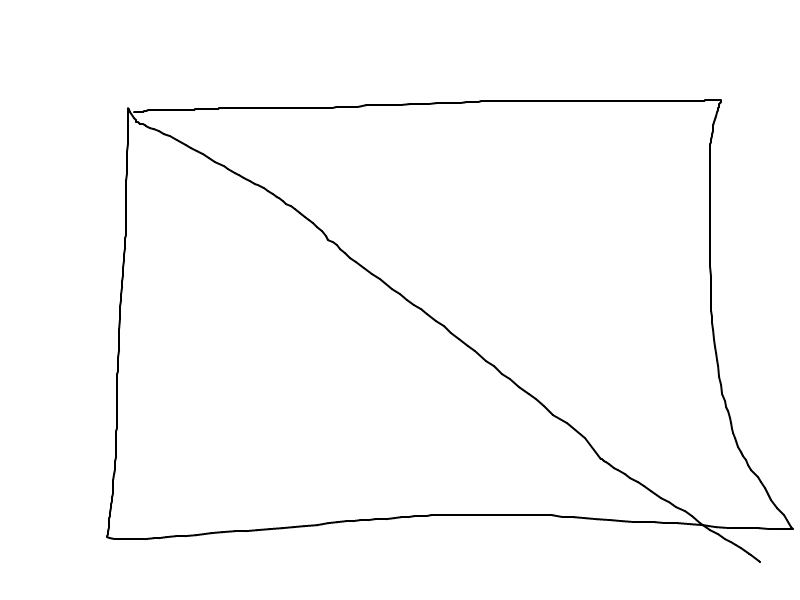
\includegraphics[scale=0.5]{pic/foo.png}
  }
  \caption{foo!!1! }
  \label{footo}
\end{figure}

Lorem ipsum.

\subsection{Wie verweist man auf Begriffe im Glossar?}

\gls{lorem} \gls{ipsum} dolor sit amet, consetetur sadipscing elitr, sed diam nonumy eirmod tempor invidunt ut labore et dolore magna aliquyam erat, sed diam voluptua. At vero eos et accusam et justo duo dolores et ea rebum. Stet clita kasd gubergren, no sea takimata sanctus est \gls{lorem} ipsum dolor sit amet. 

\section{Hauptteil}

\subsection{Quellcode-Listing mit minted}

\begin{listing}
\begin{minted}[]{java}
  for(int i = 0; i < 42; i++) {
    System.out.println(i*3.14159);
  }
\end{minted}
\end{listing}

\subsubsection{Umlaute}

Umlaute ä ö ü ß direkt anstatt durch \"a \"o \"u \ss\ oder "a "o "u "s.

ÄÖÜ

\paragraph{Hervorhebung unter subsubsection}

Das geht mit einem paragraph!

\subsubsection{Tabellen}

\begin{table}[h]
\begin{tabular}{lllll}
blabla &  At vero eos et accusam et justo duo dolores et ea rebum.\\
       & consetetur sadipscing elitr. \\
blubbblubb &  Lorem ipsum dolor sit amet.\\
       & sed diam nonumy eirmod tempor invidunt ut labore. \\	   
\end{tabular}
\end{table}	


\section{Fazit}

Lorem ipsum dolor sit amet, consetetur sadipscing elitr, sed diam nonumy eirmod tempor invidunt ut labore et dolore magna aliquyam erat, sed diam voluptua. At vero eos et accusam et justo duo dolores et ea rebum. Stet clita kasd gubergren, no sea takimata sanctus est Lorem ipsum dolor sit amet. Lorem ipsum dolor sit amet, consetetur sadipscing elitr, sed diam nonumy eirmod tempor invidunt ut labore et dolore magna aliquyam erat, sed diam voluptua. At vero eos et accusam et justo duo dolores et ea rebum. Stet clita kasd gubergren, no sea takimata sanctus est Lorem ipsum dolor sit amet.

\newpage

\section{Quellen- und Literaturverzeichnis}

\begin{thebibliography}{999}
\bibitem [wikipedia] {Wikipedia} Wikimedia Coorp: \glqq How to wiki?\grqq{} \url{http://en.wikipedia.org/wiki/wikiwikiwiki}, aufgerufen am \today{}
\end{thebibliography}

\section{Abbildungs- und Tabellenverzeichnis}

\renewcommand{\listfigurename}{Verzeichnis der Abbildungen}
\listoffigures

\newpage

\printglossary

\end{document}
